\documentclass[]{article}
\usepackage{graphicx}
\usepackage{amsmath}
\usepackage[a4paper,bindingoffset=0.2in,%
left=0.9in,right=0.9in,top=1.2in,bottom=1.2in,%
footskip=.25in]{geometry}
\usepackage{caption}
\usepackage{subcaption}
\usepackage{adjustbox}
\usepackage{tabularx}
\usepackage{rotating}
\usepackage{hyperref}

%opening
\title{A Note on GMM Estimation of Theories of Expectation Formation}
\author{Tao Wang}

\begin{document}

\maketitle

\section{A Generic Framework}

For a given process of inflation and a particular theory of expectation formation, the GMM estimate of the vector of parameters $\Omega$ is defined as the following. 

\begin{eqnarray}
\widehat \Omega = \underset{\Omega }{argmin} (M_{\textrm{data} } - F(\Omega, Y)) W  (M_{\textrm{data} } - F(\Omega, Y))'
\end{eqnarray}

\begin{itemize}
	\item  $\Omega$ is a vector of size of $k$, depending on the number of parameters to be estimated. 
	\item $M_{data}$ is the moments computed from data, i.e. mean forecasts, average forecast errors, the cross-sectional variance of forecasts (disagreement), average uncertainty, etc. Also the autocovariance of all the abovementioned.  
	
	\item $F$ is the moments that are generated from a certain theory of expectation formation and inflation process. It is a function of parameters $\Omega$ as well as the $Y$, the real-time data(including history) that is available to forecasters at each point of the time $t$. 
	\item For instance, for $T$ periods, $Y$ includes $T$  sequences of real-time inflation data of different lengths that terminate at each point of the forecasting:  $t =0$, $t=1$... $t=T$ . 
	\item  Both $M$ and $F$ is of the size  $m$, depending on the number of moments used for estimation. For instance, if we only estimate expectation formation using mean forecasts, disagreements and forecast errors while taking the inflation process as given, there are three moments, thus $m = 3$. If we include autocovariance of forecast errors, then $m=4$.  
	
	\item $W$ is the weighting matrix. For now, I stick to the identity matrix. 
\end{itemize}

The above procedure is specific to a pair of assumed inflation process and a theory of expectation. It can be estimated only for the theory of expectation formation with exogenous fed parameters of the inflation process using the entire history of inflation data, or we could jointly estimate the parameters of expectation formation and the inflation process. 

\section{Estimation}
\subsection{Real-time Data}

When agents form their expectations of inflation at any point of the time, what is potentially available to them is the real-time inflation data, namely those released from the most update-to-date vintage of the inflation. In order to match as close as possible the information set available to the forecasting agents, we need to use real-time data for each particular point of time.  

These real-time vintage inflation data since 1998 were obtained from the Real-Time Data Research Center hosted by the Federal Reserve Bank of Philadelphia. 

To get an idea of how much of the differences there are between the real-time inflation and the most recent vintage in 2018, Figure \ref{real_time_rev} and \ref{ts_real_time_current_vintage} plot, respectively, the distributions of the revisions as well as the time series of the inflation. Although overall, there is no obvious skewness of the revisions, there have been indeed sizable revisions made for the real-time data. 

\begin{figure}[htbp]
		\centering
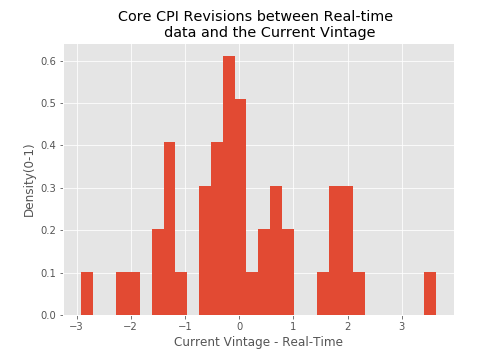
\includegraphics[width=0.7\textwidth]{figures/hist_rev_realtime.png}
\caption{Revisions of Current-vintage from Real-time Core CPI}
\label{real_time_rev}
	\begin{flushleft}
	{\footnotesize Note: real-time data  at time $t$ is defined the inflation from $t-1$ to $t$ according to the most recent vintage of CPI inflation at time $t$. The period is between 2000 M1-2018 M3.}
\end{flushleft}
\end{figure}


\begin{figure}[htbp]
	\centering
	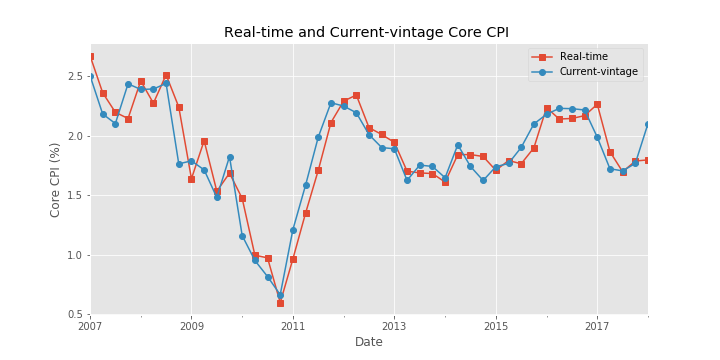
\includegraphics[width=0.8\textwidth]{figures/ts_rev_realtime.png}
	\caption{Current-vintage and Real-time Core CPI}
	\label{ts_real_time_current_vintage}
\end{figure}

\subsection{Results}

\subsubsection{Professional Forecasters}

Figure \ref{SE_diag_SPF} and \ref{SE_diag_joint_SPF} plot the estimated moments for SE model together with the data moments professional forecasts of SPF. 

From left to the right, the four columns of the figures are based on estimation using different choices of moments. 

Figure \ref{NI_diag_SPF} and \ref{NI_diag_joint_SPF} plot the estimated moments for NI model together with the data moments professional forecasts of SPF. 

\begin{figure}[ht]
	\centering
	\begin{subfigure}[b]{\textwidth}
		\centering
		\caption{Estimation of SE for Professionals}
		\label{SE_diag_SPF}
		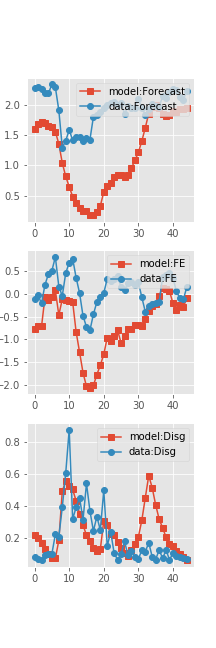
\includegraphics[width=0.19\textwidth]{figures/spf_se_est_diag0.png}
		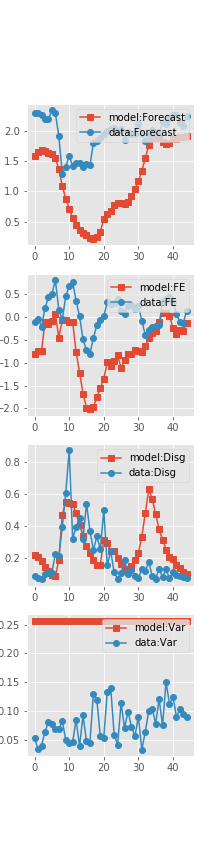
\includegraphics[width=0.19\textwidth]{figures/spf_se_est_diag1.png}
		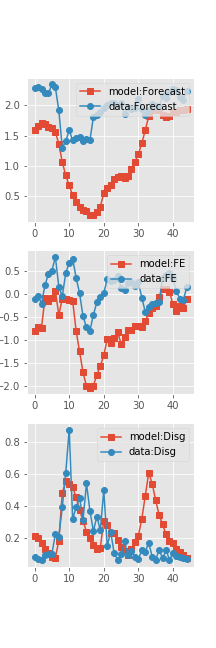
\includegraphics[width=0.19\textwidth]{figures/spf_se_est_diag2.png}
		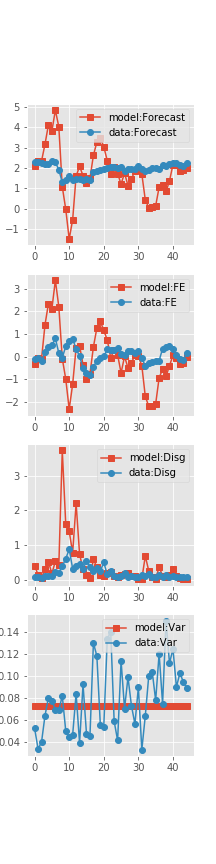
\includegraphics[width=0.19\textwidth]{figures/spf_se_est_diag3.png}
		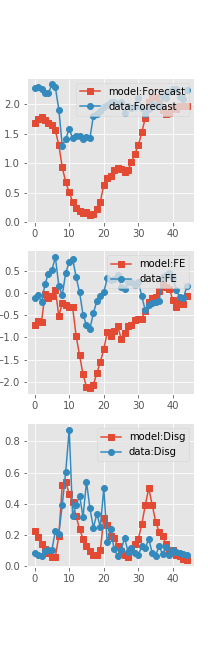
\includegraphics[width=0.19\textwidth]{figures/spf_se_est_diag4.png}
	\end{subfigure}
	\vspace{1em}
	\vfill
	\begin{subfigure}[b]{\textwidth}
		\centering
		\caption{Joint Estimation of SE and Inflation Process}
		\label{SE_diag_joint_SPF}
	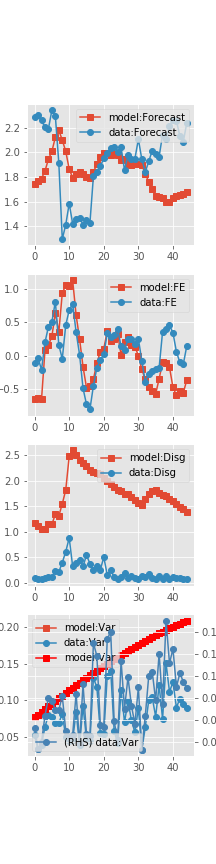
\includegraphics[width=0.19\textwidth]{figures/spf_se_est_joint_diag0.png}
	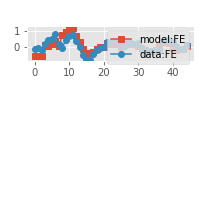
\includegraphics[width=0.19\textwidth]{figures/spf_se_est_joint_diag1.png}
	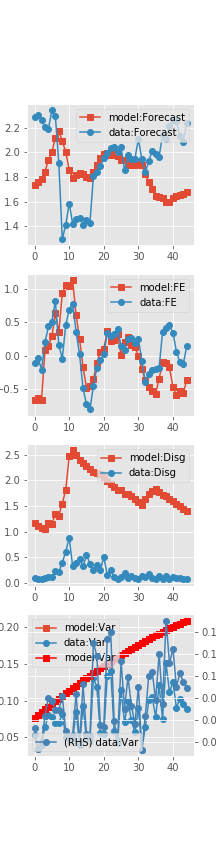
\includegraphics[width=0.19\textwidth]{figures/spf_se_est_joint_diag2.png}
	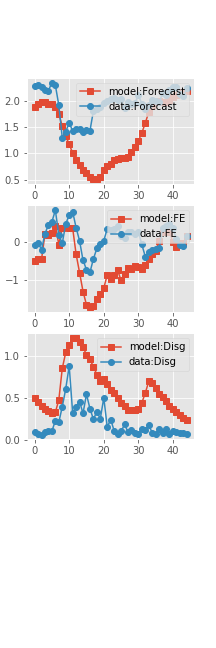
\includegraphics[width=0.19\textwidth]{figures/spf_se_est_joint_diag3.png}
	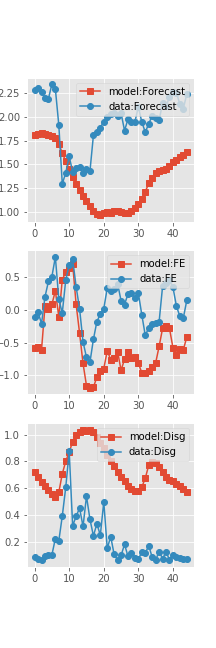
\includegraphics[width=0.19\textwidth]{figures/spf_se_est_joint_diag4.png}
	\end{subfigure}
	\\
	\begin{flushleft}
		{\footnotesize Note: the upper panel estimates expectation formation only taking the process of inflation parameters as given. The bottom panel estimates the parameters of expectation formation and inflation process jointly. From left to the right, the moments used are $\overline y_{t|t}$, $\overline{FE}_{t}$, $\overline y_{t|t}$/$\overline{FE}_{t}$ and $\overline y_{t|t}$ / $\overline{FE}_{t}$/ $\overline{\textrm{Disg}_t}$, $\overline y_{t|t}$ / $\overline{FE}_{t}$/ $\overline{\textrm{Disg}_t}$/$\overline{Var}_t$,  respectively. }
	\end{flushleft}
	\caption{SE of Professionals: Esimated Model Moments and Data Moments}
\end{figure}


\begin{figure}[ht]
	\centering
	\begin{subfigure}[b]{\textwidth}
		\centering
		\caption{Estimation of NI for Professionals}
		\label{NI_diag_SPF}
		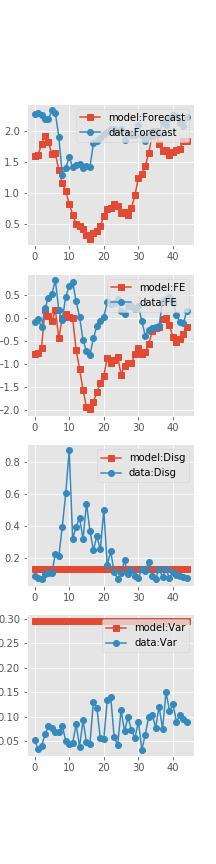
\includegraphics[width=0.19\textwidth]{figures/spf_ni_est_diag0.png}
		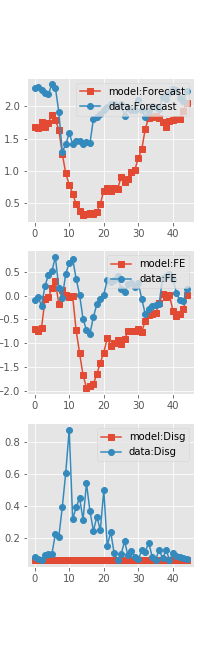
\includegraphics[width=0.19\textwidth]{figures/spf_ni_est_diag1.png}
		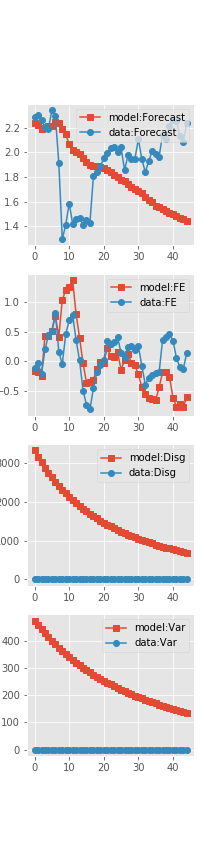
\includegraphics[width=0.19\textwidth]{figures/spf_ni_est_diag2.png}
		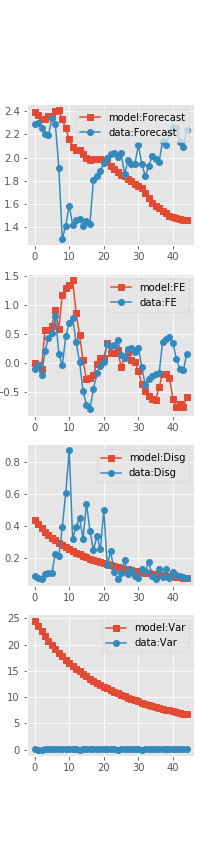
\includegraphics[width=0.19\textwidth]{figures/spf_ni_est_diag3.png}
		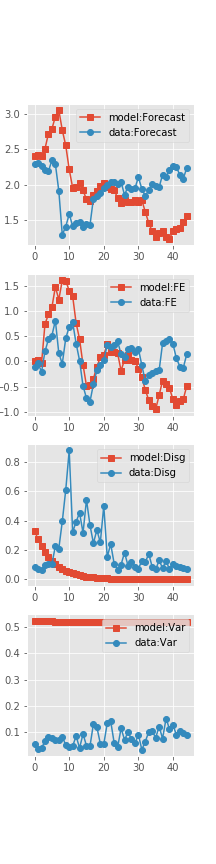
\includegraphics[width=0.19\textwidth]{figures/spf_ni_est_diag4.png}
	\end{subfigure}
	\vspace{1em}
	\vfill
	\begin{subfigure}[b]{\textwidth}
		\centering
		\caption{Joint Estimation of NI and Inflation Process}
		\label{NI_diag_joint_SPF}
		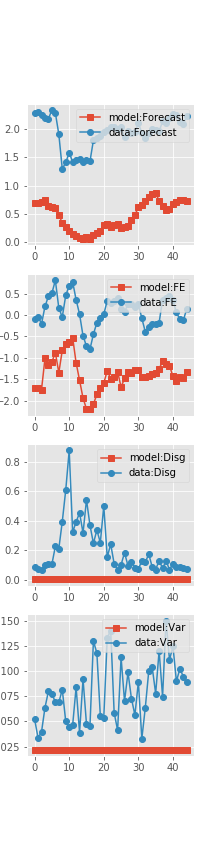
\includegraphics[width=0.19\textwidth]{figures/spf_ni_est_joint_diag0.png}
		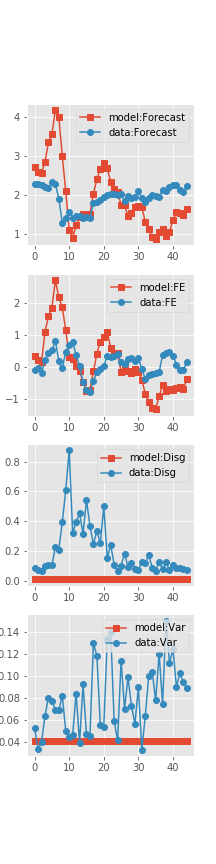
\includegraphics[width=0.19\textwidth]{figures/spf_ni_est_joint_diag1.png}
		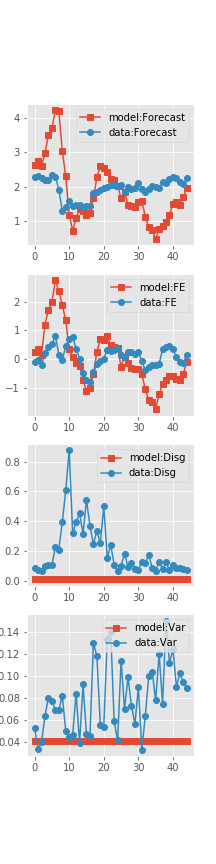
\includegraphics[width=0.19\textwidth]{figures/spf_ni_est_joint_diag2.png}
		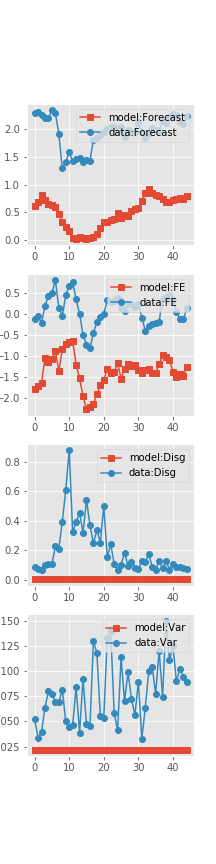
\includegraphics[width=0.19\textwidth]{figures/spf_ni_est_joint_diag3.png}
		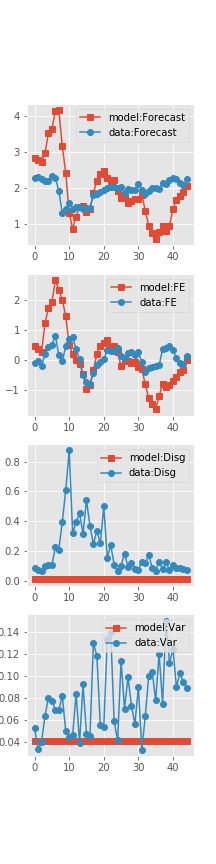
\includegraphics[width=0.19\textwidth]{figures/spf_ni_est_joint_diag4.png}
	\end{subfigure}
	\\
	\begin{flushleft}
		{\footnotesize Note: the upper panel estimates expectation formation only taking the process of inflation parameters as given. The bottom panel estimates the parameters of expectation formation and inflation process jointly. From left to the right, the moments used are $\overline y_{t|t}$, $\overline{FE}_{t}$, $\overline y_{t|t}$/$\overline{FE}_{t}$ and $\overline y_{t|t}$ / $\overline{FE}_{t}$/ $\overline{\textrm{Disg}_t}$, $\overline y_{t|t}$ / $\overline{FE}_{t}$/ $\overline{\textrm{Disg}_t}$/$\overline{Var}_t$,  respectively. }
	\end{flushleft}
	\caption{NI of Professionals: Esimated Model Moments and Data Moments}
\end{figure}

\subsubsection{Households}


Figure \ref{SE_diag_SCE} and \ref{SE_diag_joint_SCE} plot the estimated moments for SE model together with the data moments of households inflation forecasts from SCE. 

From left to the right, the four columns of the figures are based on estimation using different choices of moments. 

Figure \ref{NI_diag_SCE} and \ref{NI_diag_joint_SCE} plot the estimated moments for NI model together with the data moments of households inflation forecasts from SCE. 

\begin{figure}[htbp]
	\centering
	\begin{subfigure}[b]{\textwidth}
		\centering
		\caption{Estimation of SE for Households}
		\label{SE_diag_SCE}
		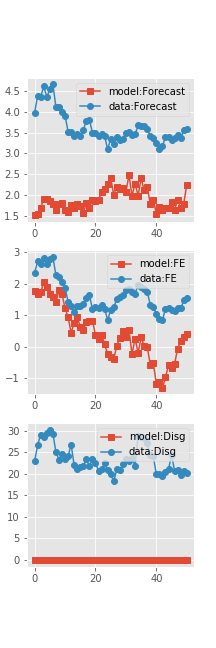
\includegraphics[width=0.19\textwidth]{figures/sce_se_est_diag0.png}
		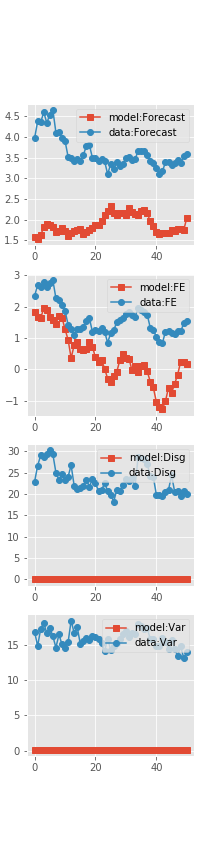
\includegraphics[width=0.19\textwidth]{figures/sce_se_est_diag1.png}
		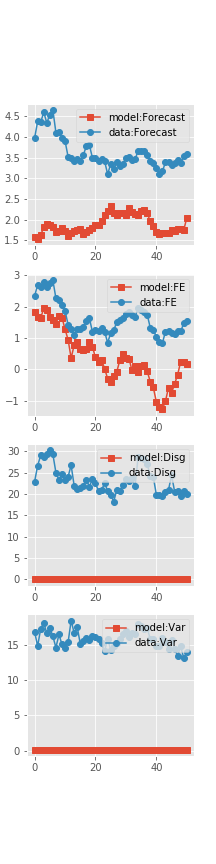
\includegraphics[width=0.19\textwidth]{figures/sce_se_est_diag2.png}
		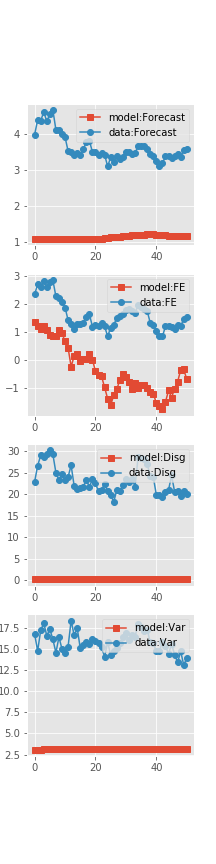
\includegraphics[width=0.19\textwidth]{figures/sce_se_est_diag3.png}
		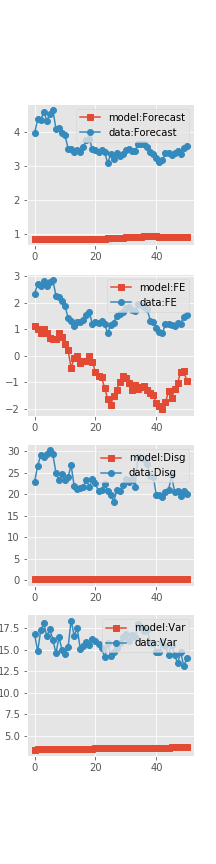
\includegraphics[width=0.19\textwidth]{figures/sce_se_est_diag4.png}
	\end{subfigure}
	\vspace{1em}
	\vfill
	\begin{subfigure}[b]{\textwidth}
		\centering
		\caption{Joint Estimation of SE and Inflation Process}
		\label{SE_diag_joint_SCE}
		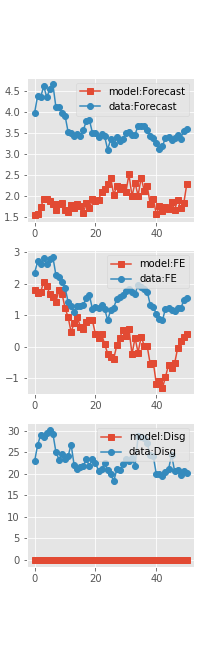
\includegraphics[width=0.19\textwidth]{figures/sce_se_est_joint_diag0.png}
		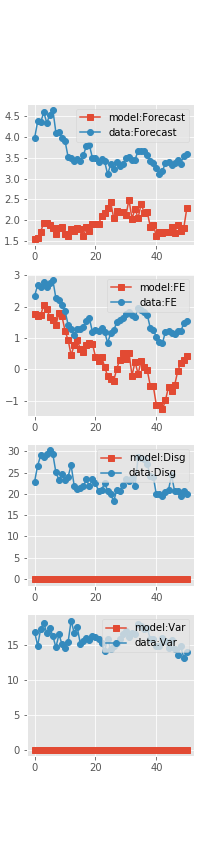
\includegraphics[width=0.19\textwidth]{figures/sce_se_est_joint_diag1.png}
		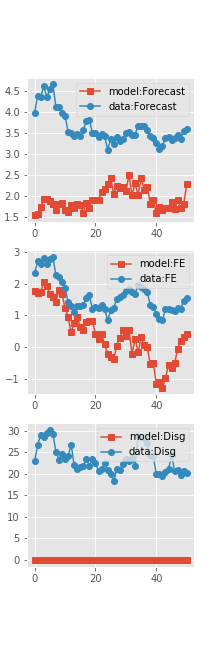
\includegraphics[width=0.19\textwidth]{figures/sce_se_est_joint_diag2.png}
		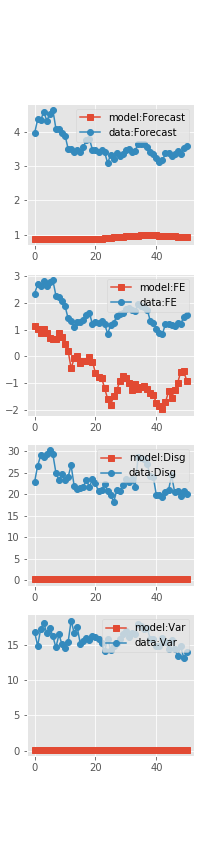
\includegraphics[width=0.19\textwidth]{figures/sce_se_est_joint_diag3.png}
		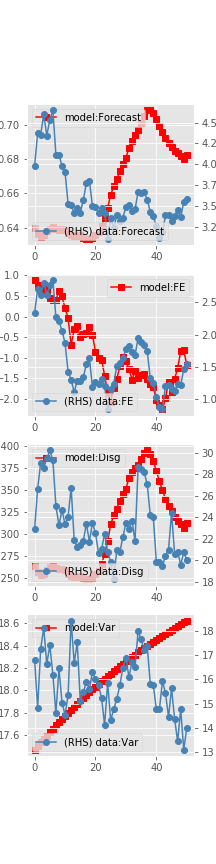
\includegraphics[width=0.19\textwidth]{figures/sce_se_est_joint_diag4.png}
	\end{subfigure}
	\\
	\begin{flushleft}
		{\footnotesize Note: the upper panel estimates expectation formation only taking the process of inflation parameters as given. The bottom panel estimates the parameters of expectation formation and inflation process jointly. From left to the right, the moments used are $\overline y_{t|t}$, $\overline{FE}_{t}$, $\overline y_{t|t}$/$\overline{FE}_{t}$ and $\overline y_{t|t}$ / $\overline{FE}_{t}$/ $\overline{\textrm{Disg}_t}$, $\overline y_{t|t}$ / $\overline{FE}_{t}$/ $\overline{\textrm{Disg}_t}$/$\overline{Var}_t$,  respectively. }
	\end{flushleft}
	\caption{SE of Households: Esimated Model Moments and Data Moments}
\end{figure}


\begin{figure}[htbp]
	\centering
	\begin{subfigure}[b]{\textwidth}
		\centering
		\caption{Estimation of NI  for Households}
		\label{NI_diag_SCE}
		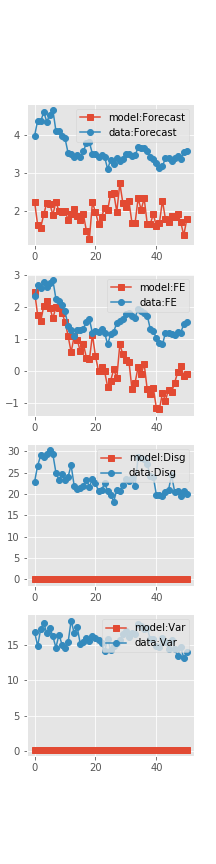
\includegraphics[width=0.19\textwidth]{figures/sce_ni_est_diag0.png}
		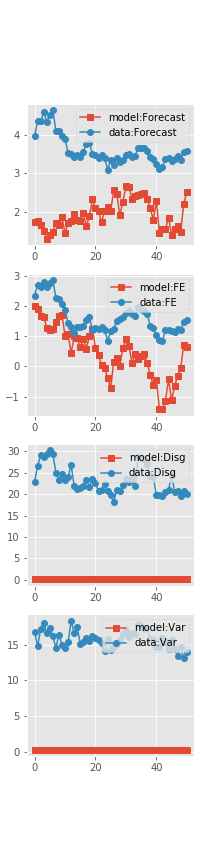
\includegraphics[width=0.19\textwidth]{figures/sce_ni_est_diag1.png}
		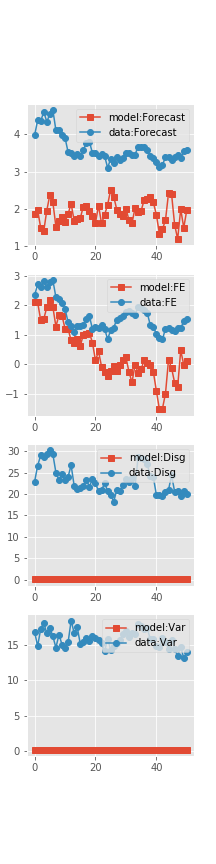
\includegraphics[width=0.19\textwidth]{figures/sce_ni_est_diag2.png}
		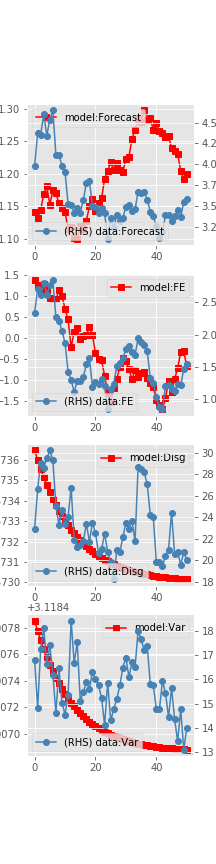
\includegraphics[width=0.19\textwidth]{figures/sce_ni_est_diag3.png}
		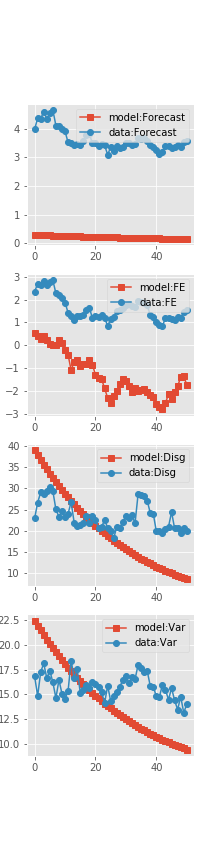
\includegraphics[width=0.19\textwidth]{figures/sce_ni_est_diag4.png}
	\end{subfigure}
	\vspace{1em}
	\vfill
	\begin{subfigure}[b]{\textwidth}
		\centering
		\caption{Joint Estimation of SE and Inflation Process}
		\label{NI_diag_joint_SCE}
		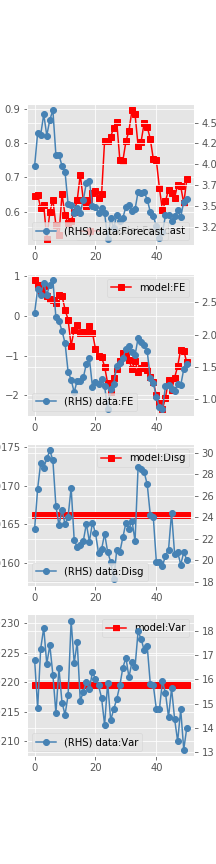
\includegraphics[width=0.19\textwidth]{figures/sce_ni_est_joint_diag0.png}
		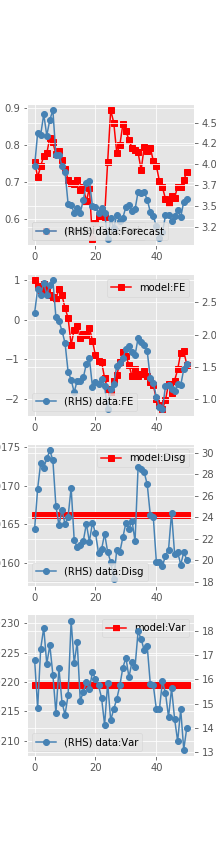
\includegraphics[width=0.19\textwidth]{figures/sce_ni_est_joint_diag1.png}
		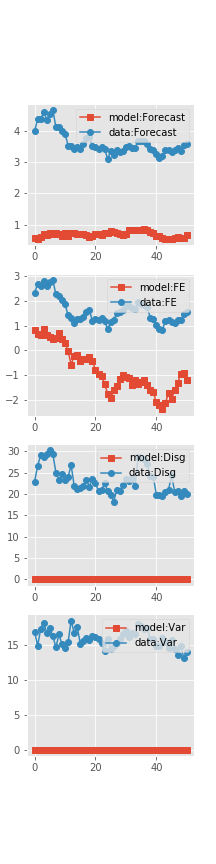
\includegraphics[width=0.19\textwidth]{figures/sce_ni_est_joint_diag2.png}
		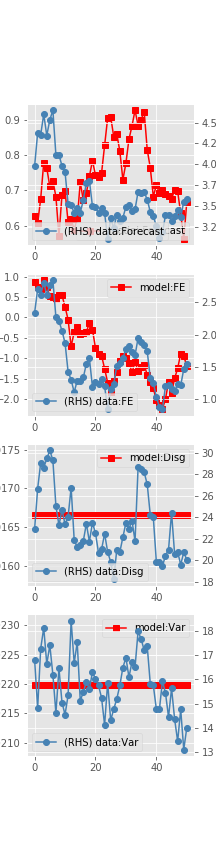
\includegraphics[width=0.19\textwidth]{figures/sce_ni_est_joint_diag3.png}
		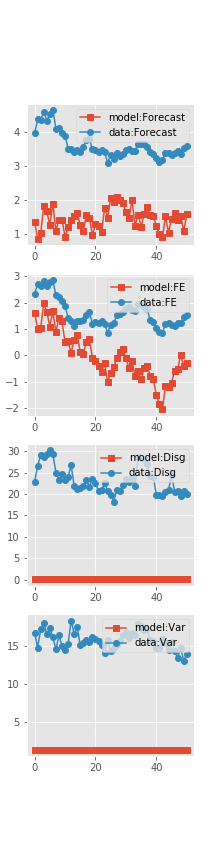
\includegraphics[width=0.19\textwidth]{figures/sce_ni_est_joint_diag4.png}
	\end{subfigure}
	\\
	\begin{flushleft}
		{\footnotesize Note: the upper panel estimates expectation formation only taking the process of inflation parameters as given. The bottom panel estimates the parameters of expectation formation and inflation process jointly. From left to the right, the moments used are $\overline y_{t|t}$, $\overline{FE}_{t}$, $\overline y_{t|t}$/$\overline{FE}_{t}$ and $\overline y_{t|t}$ / $\overline{FE}_{t}$/ $\overline{\textrm{Disg}_t}$, $\overline y_{t|t}$ / $\overline{FE}_{t}$/ $\overline{\textrm{Disg}_t}$/$\overline{Var}_t$,  respectively.  }
	\end{flushleft}
	\caption{NI of Households: Esimated Model Moments and Data Moments}
\end{figure}

	\begin{sidewaystable}[t]
		\centering
	\caption{GMM Estimates of Parameters of SE and Inflation Process}
	\label{GMM_Est_SE_Table}
\begin{tabular}{llllllllllll}
	\hline 
	0        & 1  & 2    & 3   & SE: $\hat\lambda_{SPF}$(Q) & SE: $\hat\lambda_{SPF}$(Q) & SE: $\rho$ & SE: $\sigma$ & SE: $\hat\lambda_{SCE}$(M) & SE: $\hat\lambda_{SCE}$(M) & SE: $\rho$ & SE: $\sigma$ \\
	\hline 
	Forecast &    &      &     & 0.21                       & 0.01                       & 1          & 0.1          & 1                          & 1                          & 1          & 0.1          \\
	\hline 
	FE       &    &      &     & 0.18                       & 0.01                       & 1          & 0.1          & 1                          & 1                          & 1          & 0.1          \\
	\hline 
	Forecast & FE &      &     & 0.2                        & 0.01                       & 1          & 0.1          & 1                          & 1                          & 1          & 0.1          \\
	\hline 
	Forecast & FE & Disg &     & 0.23                       & 0.05                       & 1          & 0.1          & 0.02                       & 0.03                       & 0.98       & 0.1          \\
	\hline 
	Forecast & FE & Disg & Var & 0.26                       & 0.05                       & 1          & 0.07         & 0.01                       & 0.03                       & 0.98       & 1.11        \\
	\hline 
\end{tabular}
\end{sidewaystable}


\begin{sidewaystable}[t]
	\centering
	\caption{GMM Estimates of Parameters of NI and Inflation Process}
	\label{GMM_Est_NI_Table}
\begin{tabular}{llllllllllllllll}
	\hline 
	0        & 1  & 2    & 3   & NI: $\hat\sigma_{pb,SPF}$ & $\hat\sigma_{pr,SPF}$ & NI: $\hat\sigma_{pb,SPF}$ & $\hat\sigma_{pr,SPF}$ & NI: $\rho$ & NI: $\sigma$ & NI: $\hat\sigma_{pb,SCE}$ & $\hat\sigma_{pr,SCE}$ & NI: $\hat\sigma_{pb,SCE}$ & $\hat\sigma_{pr,SCE}$ & NI: $\rho$ & NI: $\sigma$ \\
	\hline 
	Forecast &    &      &     & 376.66                    & 1.26                  & 0.5                       & 0.5                   & 0.8        & 0.1          & 0                         & 1.13                  & 0.5                       & 0.5                   & 0.8        & 0.1          \\
	\hline 
	FE       &    &      &     & 1.04                      & 159.74                & 0.5                       & 0.5                   & 0.8        & 0.1          & 0                         & 1.26                  & 0.5                       & 0.5                   & 0.8        & 0.1          \\
	\hline 
	Forecast & FE &      &     & 1.14                      & 6.74                  & 0.5                       & 0.5                   & 0.8        & 0.1          & 0.59                      & 0.36                  & 0.5                       & 0.5                   & 0.8        & 0.1          \\
	\hline 
	Forecast & FE & Disg &     & 1.39                      & 1.46                  & 0.5                       & 0.5                   & 0.8        & 0.1          & 2354.37                   & 10.93                 & 0.5                       & 0.5                   & 0.8        & 0.1          \\
	\hline 
	Forecast & FE & Disg & Var & 1.37                      & 1.1                   & 0.5                       & 0.5                   & 0.8        & 0.1          & 35263.31                  & 332.04                & 0.5                       & 0.5                   & 0.8        & 0.1         \\
	\hline 
\end{tabular}
\end{sidewaystable}

\section{Stochastic volatility model of inflation}

\subsection{Process of inflation}

Assume that the inflation follows a process of unobserved components model with stochastical volatility. 

\begin{eqnarray}
\begin{split}
& y_t = \tau_t + \eta_t,\quad \textrm{where } \eta_t =\sigma_{\eta,t} \xi_{\eta,t} \\
& \tau_t = \tau_{t-1} + \epsilon_t, \quad \textrm{where }  \epsilon_t =\sigma_{\epsilon,t} \xi_{\epsilon,t} \\
& \log\sigma^2_{\eta,t} = \log\sigma^2_{\eta,t-1} + \mu_{\eta,t} \\
& \log\sigma^2_{\epsilon,t} = \log\sigma^2_{\epsilon,t-1} + \mu_{\epsilon,t} 
\end{split}
\end{eqnarray}

The distributions of shocks to levels of the components and their volatilities are, respectively, the following.

\begin{eqnarray}
\begin{split}
& \xi_t =[\xi_{\eta,t},\xi_{\epsilon,t}] \sim N(0,I_2) \\
& \mu_{t} = [\mu_{\eta,t},\mu_{\epsilon,t}]' \sim N(0,\gamma I_2) 
\end{split}
\end{eqnarray}

The only parameter of the model is $\gamma$, which determines the time-varying volatilities. 

\subsection{Different models of expectation formation}

\subsubsection{Rational expectation}

At the point of time $t$, the RE agent sees the realization of all stochastic variables above with subscript $t$, $t-1$, etc, including $y_t$, $\tau_t$, $\eta_t$, $\sigma_{\eta,t}$, $\sigma_{\epsilon,t}$ and their realizations in the whose past. Again, $*$ stands for FIRE benchmark. 

\begin{eqnarray}
\begin{split}
\hat y^*_{t+h|i,t} & =  E^*_{i,t}(y_{t+h}|I_{i,t}) = \tau_t 
\end{split}
\end{eqnarray}

Conditional h-step-ahead variance, uncertainty is

\begin{eqnarray}
\begin{split}
Var^*_{t+h|i,t} & = \sum^{h}_{t=0} E_{i,t}(\sigma^2_{\eta,t+h}) +  E_{i,t}(\sigma^2_{\epsilon,t+h})  \\
& = \sum^{h}_{t=1} E_{i,t}(exp^{\log \sigma^2_{\eta,t}+\sum^h_{t=1}\mu_{\eta,t+h}}) +  E_{i,t}(exp^{\log \sigma^2_{\epsilon,t}+\sum^h_{t=0}\mu_{\epsilon,t+h}} ) \\
& = \sigma^2_{\eta,t} \sum^{h}_{t=0} E_{i,t}(exp^{\sum^h_{t=1}\mu_{t+h,\eta}}) +  \sigma^2_{\epsilon,t} E_{i,t}(exp^{\sum^h_{t=1}\mu_{\epsilon,t+h}} ) \\
& = \sigma^2_{\eta,t} \sum^{h}_{t=0} exp^{E_{i,t}({\sum^h_{t=1}\mu_{t+h,\eta}})- 0.5Var_{i,t}(\sum^h_{t=1}\mu_{t+h,\eta})} +  \sigma^2_{\epsilon,t} E_{i,t}(exp^{\sum^h_{t=1}\mu_{\epsilon,t+h}} ) \\
& = \sigma^2_{\eta,t} \sum^{h}_{t=0} exp^{- 0.5h\gamma_{\eta}} +  \sigma^2_{\epsilon,t} exp^{- 0.5h\gamma_{\epsilon}}  \\
\end{split} 
\end{eqnarray}

For instance, set $h=0$, the conditional volatility for the current inflation is 


\begin{eqnarray}
\begin{split}
Var^*_{t|i,t} =  \sigma^2_{\eta,t}  +  \sigma^2_{\epsilon,t}
\end{split} 
\end{eqnarray}

\end{document}
